\documentclass[conference]{IEEEtran}
\IEEEoverridecommandlockouts
% The preceding line is only needed to identify funding in the first footnote. If that is unneeded, please comment it out.
\usepackage{cite}
\usepackage{amsmath,amssymb,amsfonts}
\usepackage{algorithmic}
\usepackage{graphicx}
\usepackage{hyperref}
\usepackage{textcomp}
\usepackage{xcolor}
\usepackage{balance}
% balance columns on lastpage
% better than \flushend according to
% https://texfaq.org/FAQ-balance
%\usepackage{flushend}
\def\BibTeX{{\rm B\kern-.05em{\sc i\kern-.025em b}\kern-.08em
    T\kern-.1667em\lower.7ex\hbox{E}\kern-.125emX}}
\begin{document}

\title{Impact of Long-Term Average Soiling and Temporal Resolution on Energy Yield Analysis}

\author{\IEEEauthorblockN{Mark A. Mikofski, Umay Akkoseoglu, Javier Lopez Lorente and Usgal Zandanbal}
	\IEEEauthorblockA{DNV Energy USA, Oakland, CA 94612, USA}}

\maketitle

\begin{abstract}
Soiling losses from dust and snow are important in forecasting long-term average (LTA) energy production of photovoltaic (PV) systems. Monthly soiling profiles of dust or snow are often derived from the LTA of individual years in the historical weather data. However, irradiance and other inputs differ each year and within each year. Contradictions both in inter-annual and intra-annual weather may cause errors in predictions of LTA performance. This study investigates the magnitude of these errors from dust soiling only (not snow) by comparing annual energy production between daily versus monthly and between LTA versus individual-year monthly soiling profiles. We found a negligible delta in annual energy between monthly versus daily soiling profiles. However, we observed a bias between LTA versus individual-year monthly profiles. On average monthly LTA was 2\% to 4\% greater than individual-year monthly profiles for both a tracker and fixed tilt system at two test sites studied in the western United States. In future work, we will broaden the study to more geographical regions and compare energy predicted using historical weather versus typical meteorological year (TMY).
\end{abstract}

\begin{IEEEkeywords}
soiling, weather, energy
\end{IEEEkeywords}

\section{Introduction}
Soiling causes energy losses by reducing effective irradiance. Systems with low rainfall build up more dust soiling causing more losses, and rainfall above a threshold reduces losses. The rate at which dust soiling builds up at a site can be determined by measuring soiling ratios onsite and extracting the build-up rate and rainfall cleaning threshold empirically. These inputs can be combined with rainfall data to estimate the dust soiling loss. Often this loss is aggregated monthly and assumed uniform over the month. This monthly profile differs from daily profiles as shown in the top panel of Fig.~\ref{twentynine_palms}. Irradiance and other model inputs are hourly, and the contradiction in temporal resolution between monthly soiling and hourly inputs causes errors as shown in the bottom panel of Fig.~\ref{twentynine_palms}.

To predict the long-term average (LTA) energy production, we calculate the dust soiling losses with historical weather and derive the LTA for each month according to Eq. \ref{lta}. This LTA monthly dust soiling profile is combined with the TMY weather to calculate the LTA energy production. The individual-year monthly soiling profiles differ from the average as shown in Fig. \ref{soiling_lta}. Therefore, when evaluating energy using historical weather, using the LTA monthly soiling profile introduces errors.

\begin{equation}
\mathit{LTA}_{\mathit{month}_j}=\frac{\sum_{\mathit{year}_i={\mathit{year}_0}}^{\mathit{year}_N}{\mathit{soiling}_{\left({\mathit{year}_i},{\mathit{month}_j}\right)}}}{N} \label{lta}
\end{equation}

\begin{figure}[htbp]
\centerline{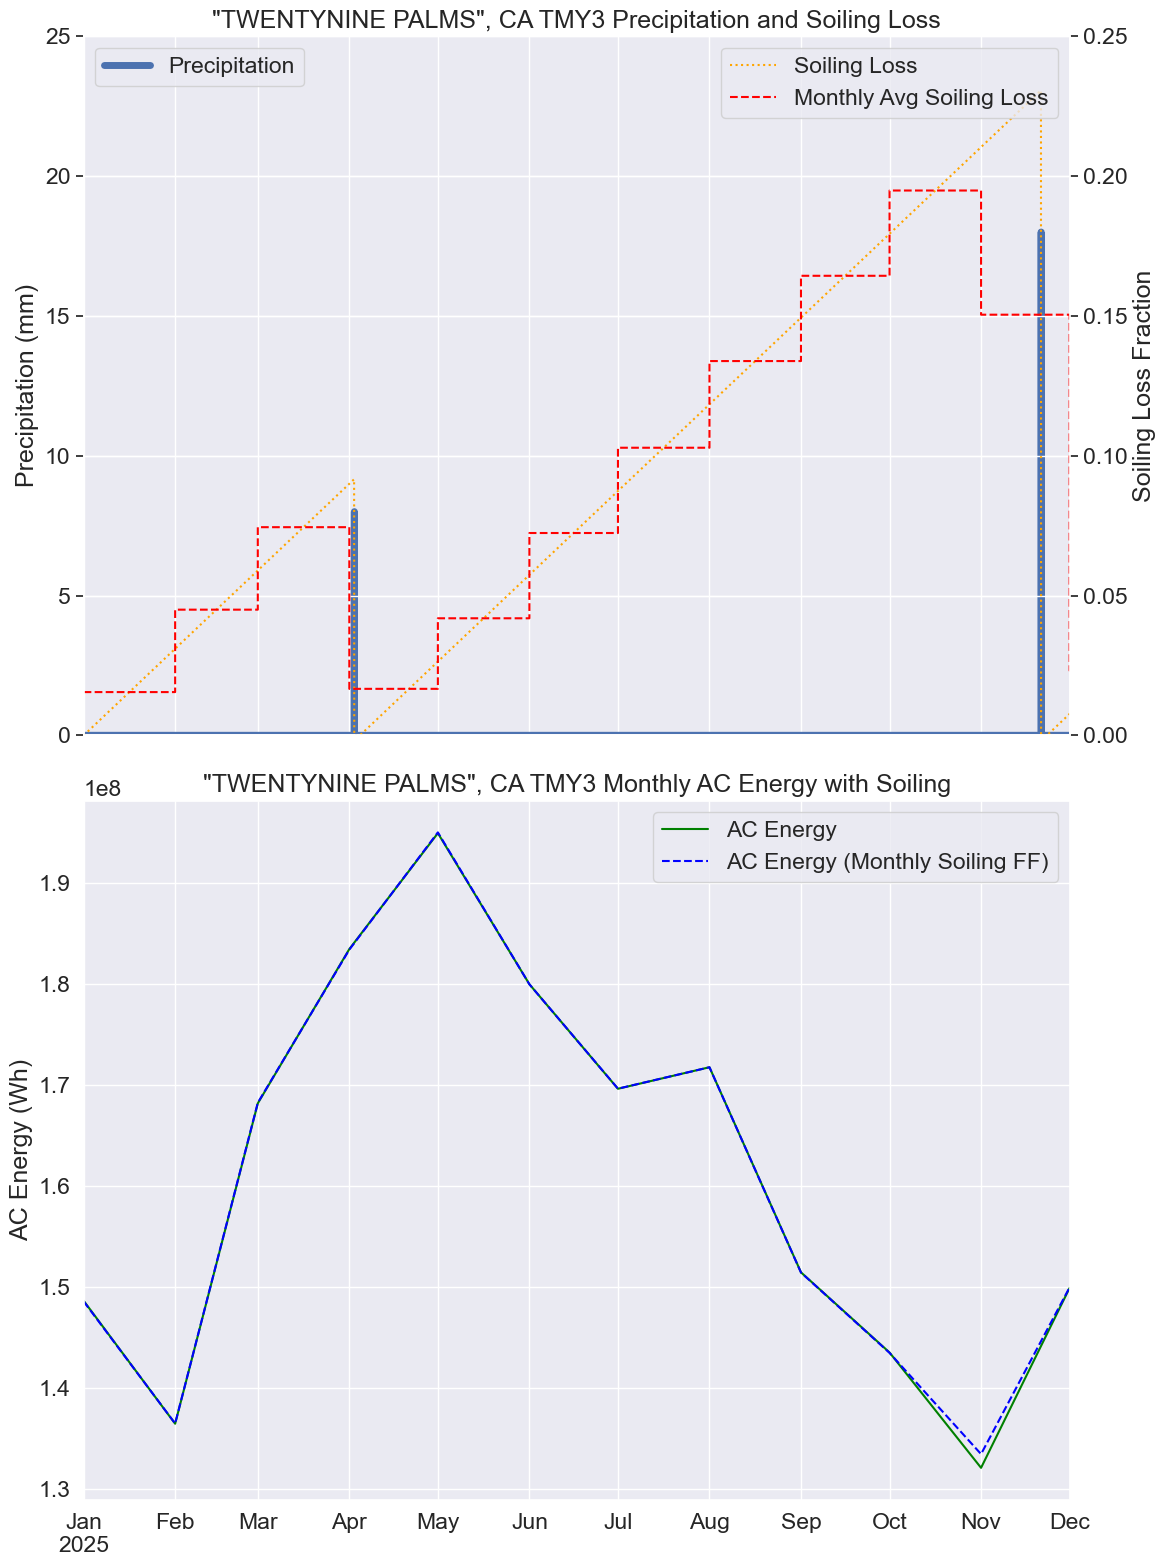
\includegraphics[width=\linewidth]{twentynine_palms.png}}
\caption{Daily and monthly soiling profiles shown at Twentynine Palms, CA (top). The monthly soiling profile is 0.1\% greater than the daily soiling profile (bottom).}
\label{twentynine_palms}
\end{figure}

\begin{figure}[htbp]
\centerline{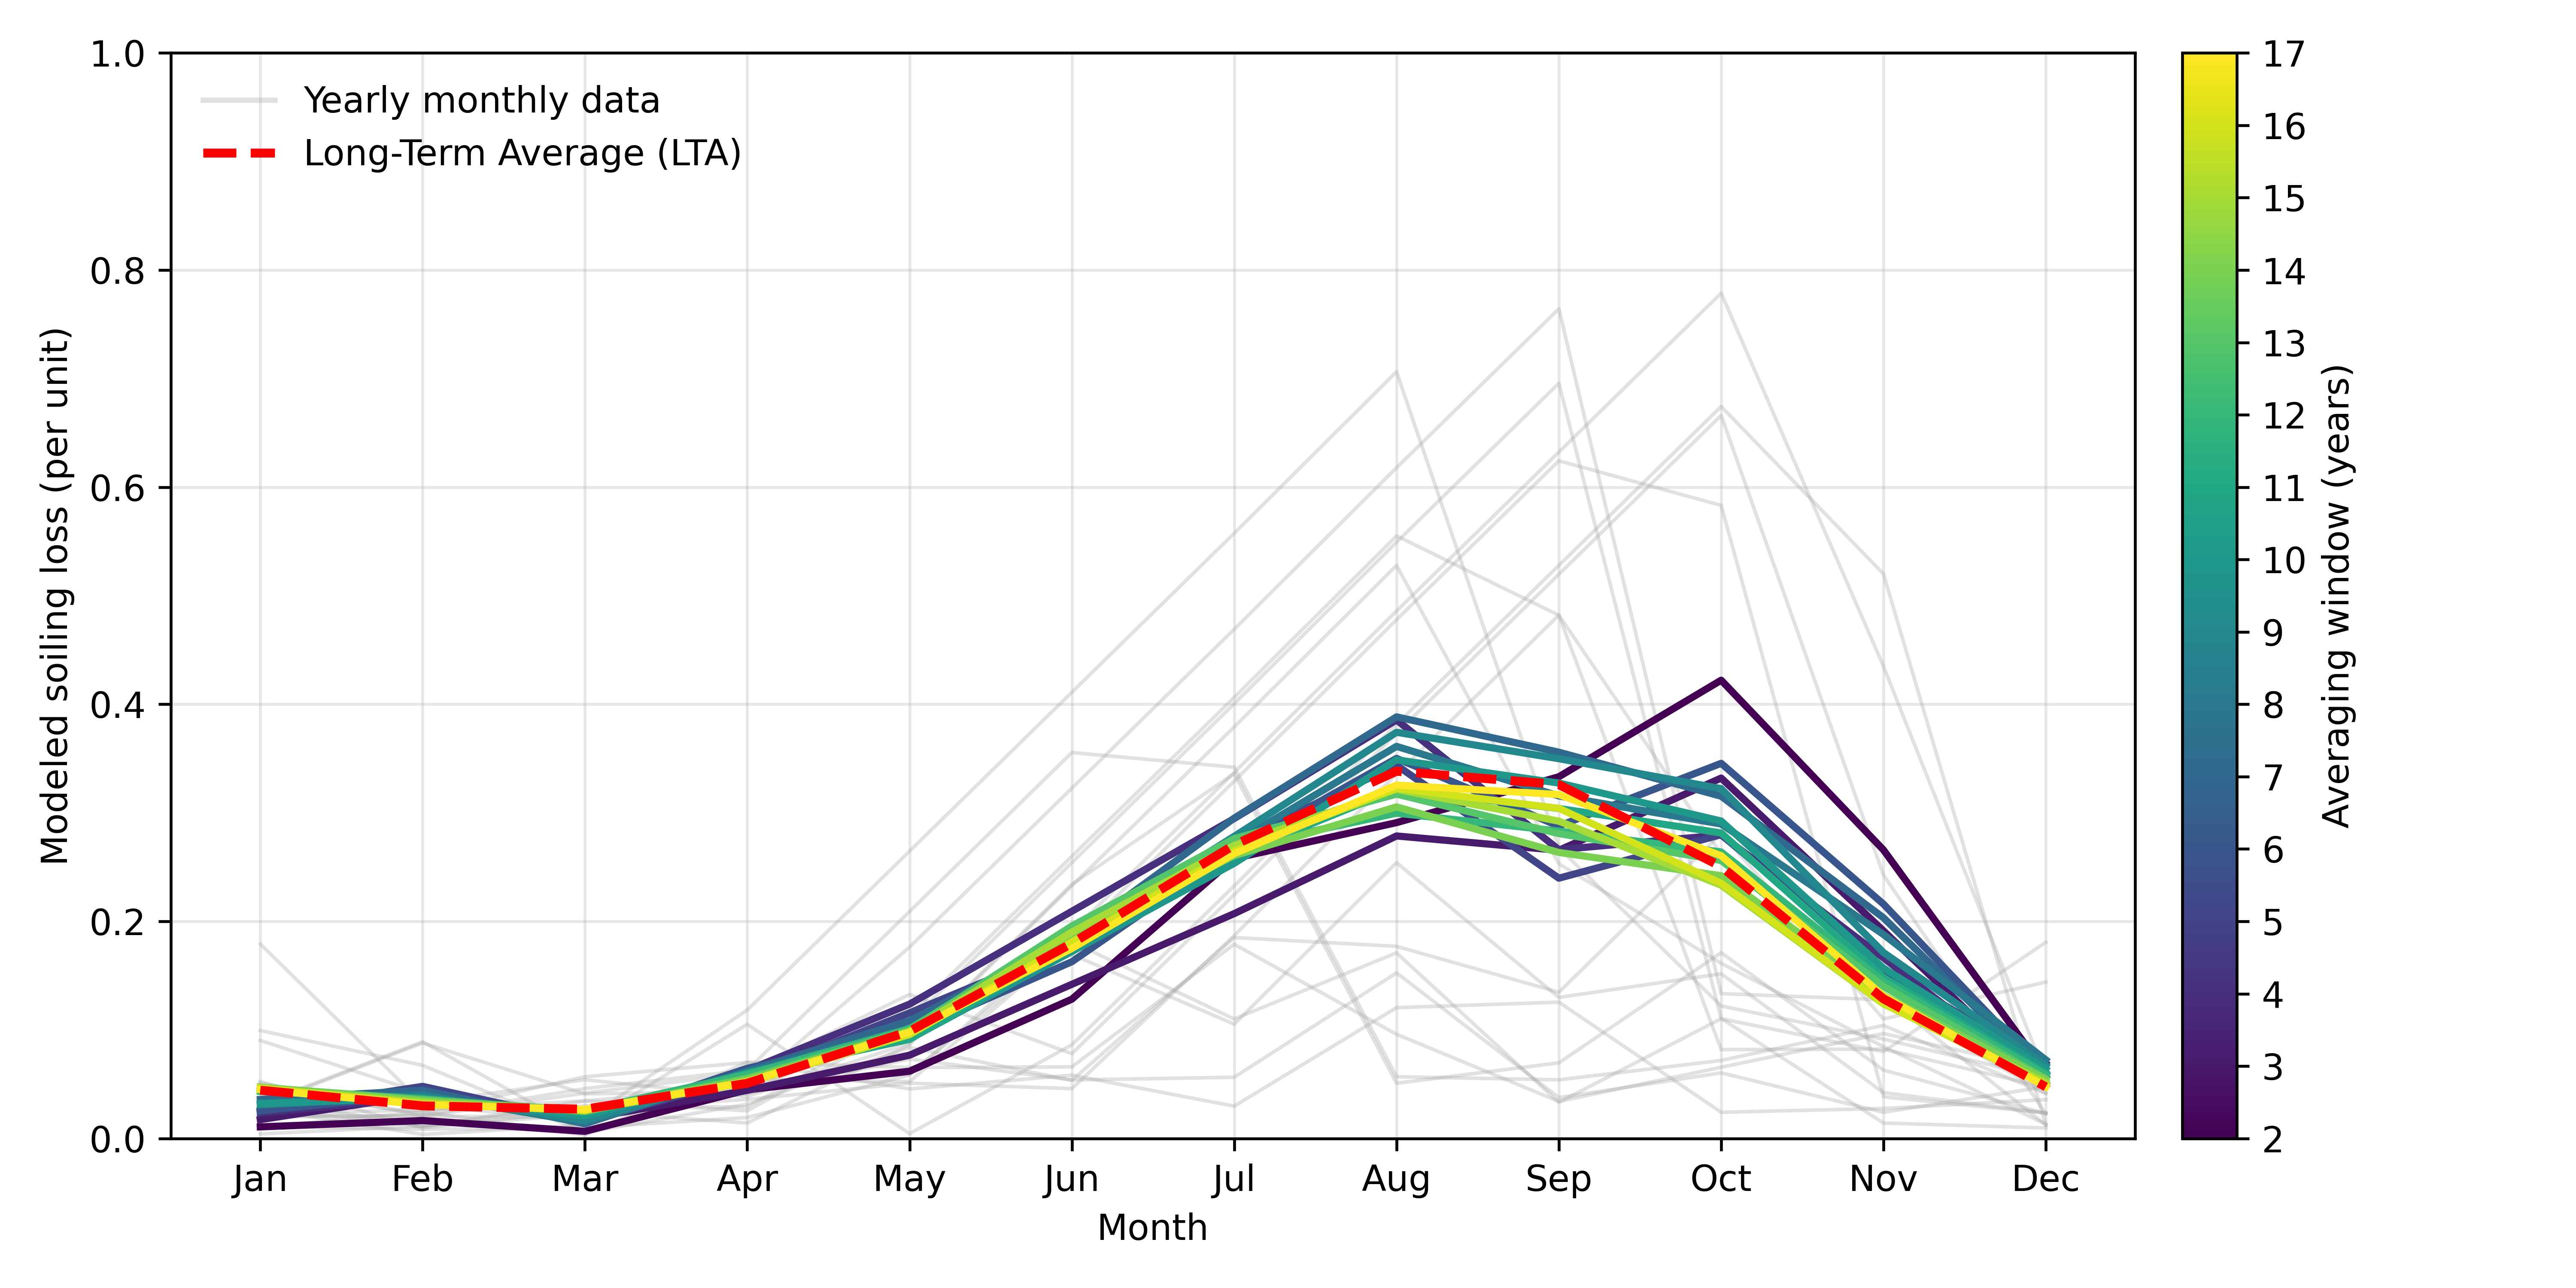
\includegraphics[width=\linewidth]{monthly_variation_rollback_kimber.png}}
\caption{Individual-year monthly soiling profiles deviate from the LTA monthly soiling profile.}
\label{soiling_lta}
\end{figure}

\section{Methods}

\subsection{Initial Study - Daily vs. Monthly}

We first investigated errors between monthly and daily dust soiling profiles. We used the Kimber soiling model \cite{kimber} from the pvlib Python package \cite{holmgren2018joss}. The following inputs were used:
\begin{itemize}
\item daily build-up rate = 0.10\%/day
\item rainfall cleaning threshold = 4-mm
\item grace days = 1-day
\end{itemize}
These inputs differ from the defaults to represent values for a broader range of geographical regions. A daily build-up rate of 0.10\%/day is used for this initial study. The rainfall cleaning threshold used was 4-mm and grace days were reduced to 1-day only. The NSRDB TMY3 dataset is used for hourly irradiance, air temperature, pressure, and rainfall. This dataset has 1000 projects located across the United States with diverse geographical and climatic conditions. The rainfall and soiling inputs are used in the Kimber model to calculate the daily soiling losses, which are aggregated monthly and then backfilled to the beginning of each month as shown in the top panel of Fig.~\ref{twentynine_palms}.

The DC and AC energy are calculated using pvwatts model chain in pvlib with Hay-Davies transposition. The irradiance, air temperature, and pressure from NSRDB are used to calculate the solar position, cell temperature, and plane-of-array (POA) global irradiance. For this initial study, we assumed a fixed-tilt of 30\textdegree\ and oriented the system due south (an azimuth of 180\textdegree). Future studies will also examine trackers systems, as well as use different soiling models like Humbolt State University (HSU) model \cite{hsu} that can calculate soiling losses as a function of module tilt. The product of the soiling loss and the global POA is the effective irradiance, which is then used in pvwatts to determine the DC and AC energy. A Jupyter notebook of the analysis is available on GitHub at https://github.com/mikofski/pvsc54-temporal-soiling-impact.

\subsection{Monthly LTA vs. Individual-Year Profiles}

Next we examined errors from combining monthly LTA dust soiling profiles with historical weather. We predicted annual energy for a both fixed-tilt and tracker systems in California with 18-years of historical weather from 2008 to 2025. We compared the energy production between monthly LTA versus individual-year dust soiling profiles with both the Kimber and Humbolt State University (HSU) soiling models as shown in Fig.~\ref{ca_kimber} and Fig.~\ref{ca_hsu} respectively.

\begin{figure}[htbp]
\centerline{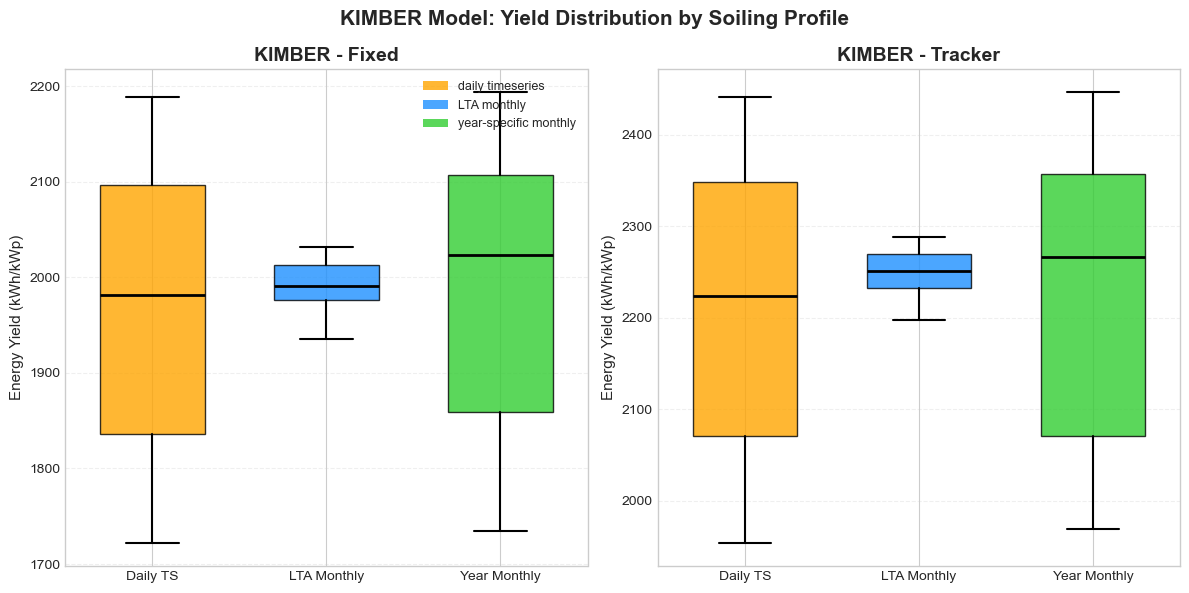
\includegraphics[width=\linewidth]{california_kimberbox.png}}
\caption{Energy production comparison between monthly LTA, individual-year, and daily dust soiling profiles from Kimber model for fixed-tilt (left) and tracker (right) systems.}
\label{ca_kimber}
\end{figure}

\begin{figure}[htbp]
\centerline{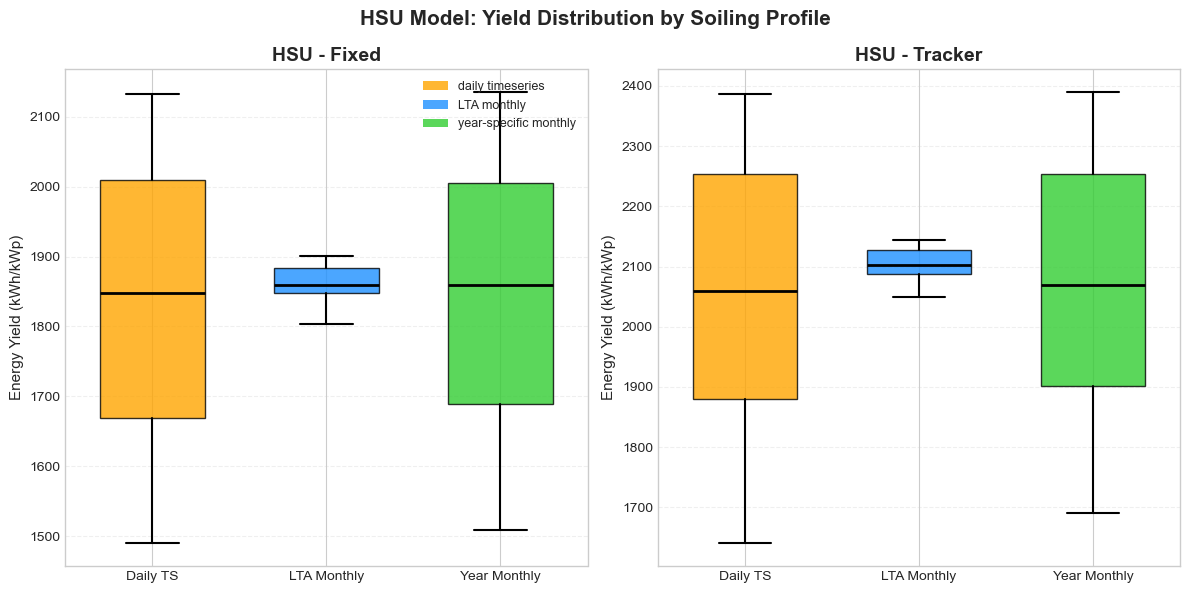
\includegraphics[width=\linewidth]{california_hsubox.png}}
\caption{Energy production comparison between monthly LTA, individual-year, and daily dust soiling profiles from HSU model for fixed-tilt (left) and tracker (right) systems.}
\label{ca_hsu}
\end{figure}


\section{Results and Discussion}

\subsection{Initial Study - Daily vs. Monthly}

We plot a histogram of the results from all the NSRDB TMY3 sites in Fig \ref{histogram}. The relative difference ($\Delta$) is calculated according to Eq.\ref{reldiff}. A negative delta means that annual energy from monthly soiling loss is larger than from daily soiling loss. The average delta for all 1000 TMY3 sites is 0.02\% and the median is 0.01\%.

\begin{equation}
\Delta=1-\frac{monthly}{daily}\label{reldiff}
\end{equation}

\begin{figure}[htbp]
\centerline{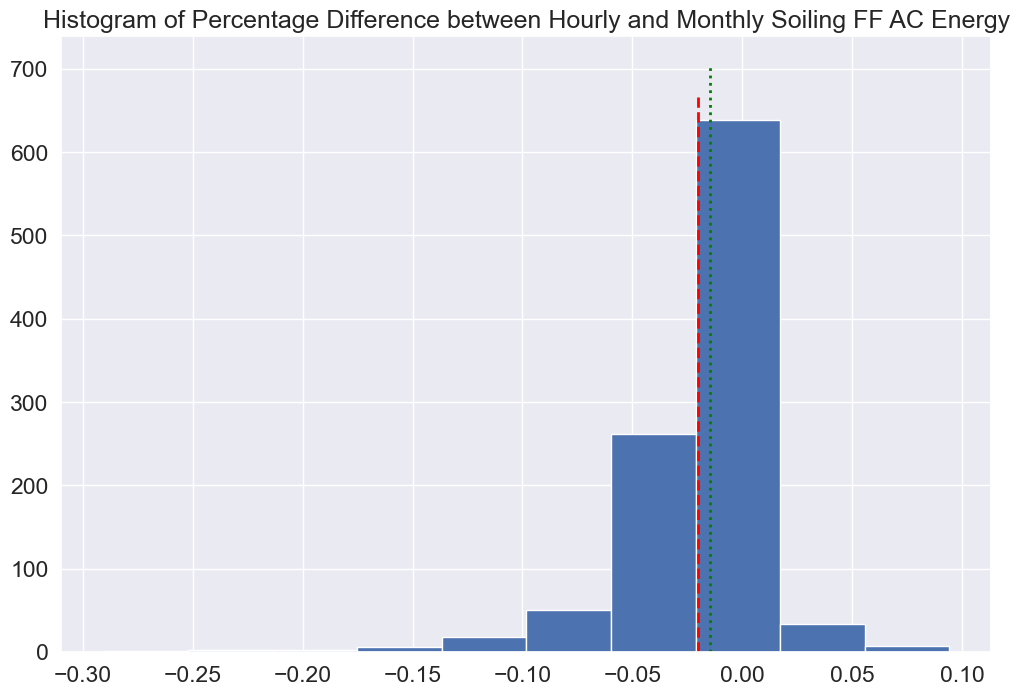
\includegraphics[width=\linewidth]{histogram.png}}
\caption{Relative difference in annual energy between monthly and daily soiling losses for all sites in NSRDB TMY3. On average there is a -0.02\% error. Negative values mean monthly is bigger, so this means that using monthly soiling profiles over predicts energy, but by a negligible amount according to this initial study.}
\label{histogram}
\end{figure}

We don't want to draw too many conclusions from this initial study, but we observed that sites with low rainfall like Twentynine Palms have a larger error between monthly and daily soiling losses. However, the error, only -0.1\% is still negligible. Overall more than 95\% of the sites have an error between monthly and daily soiling loss of less than -0.1\% which is small compared to the annual soiling loss over all, which is on the order of 2\% or more. 

\subsection{Monthly LTA vs. Individual-Year Profiles}

The energy production comparisons shown in Fig.~\ref{ca_kimber} and Fig.~\ref{ca_hsu} show large variations when the monthly LTA dust soiling profile is used with historical timeseries data due to inter-annual variability between individual years regardless of the dust soiling model (Kimber vs. HSU) or PV system type (fixed-tilt vs. tracker). For Kimber, we observe a bias both between daily vs. monthly and between individual-year and monthly LTA. However, for HSU the difference between individual-year and daily timeseries is much smaller, similar to the results of the comparison between daily and monthly dust soiling with NSRDB TMY3. We speculate the difference between Kimber and HSU may be caused by the constant ramp rate in Kimber, while HSU ramp rate varies depending on changing concentration of particulate matter (PM). There is still a bias between the monthly LTA profiles and both daily timeseries and individual-year monthly profiles. Therefore, when using historical weather, we recommend daily soiling profile derived from the individual-year timeseries to reduce forecasting errors.

\balance
\section{Conclusion and Future Work}

We investigated errors in annual energy caused by temporal differences between monthly versus daily and between monthly LTA vs. individual-year dust soiling profiles. In the first part of this initial study, we assumed a fixed tilt system to evaluate with 1000 TMY3 locations form the NSRDB. The average error was -0.02\% which is 100-times smaller than a typical annual soiling loss, and therefore we believe can be assumed negligible. However, this study is limited to a single model (Kimber), a single PV system configuration, and a single TMY year. In the final report, we will analyze tracker systems, compare monthly and daily soiling loss with HSU model, and evaluate inter-annual variability as well. In the second part of this study we compared monthly LTA vs. individual-year dust soiling profiles with historical weather and observed a bias when using monthly LTA dust soiling profiles. In a future study, we will compare the observed bias to LTA energy forecast with TMY and monthly LTA dust soiling profiles.

\begin{thebibliography}{00}
\bibitem{kimber}
A. Kimber, L. Mitchell, S. Nogradi and H. Wenger, "The Effect of Soiling on Large Grid-Connected Photovoltaic Systems in California and the Southwest Region of the United States," 2006 IEEE 4th World Conference on Photovoltaic Energy Conference, Waikoloa, HI, USA, 2006, pp. 2391-2395, doi: 10.1109/WCPEC.2006.279690.
\bibitem{hsu}
M. Coello and L. Boyle, “Simple Model For Predicting Time Series Soiling of Photovoltaic Panels,” in IEEE Journal of Photovoltaics. DOI: 10.1109/JPHOTOV.2019.2919628
\bibitem{holmgren2018joss}
Anderson, K., Hansen, C., Holmgren, W., Jensen, A., Mikofski, M., and Driesse, A. “pvlib python: 2023 project update.” Journal of Open Source Software, 8(92), 5994, (2023). DOI: 10.21105/joss.05994.
\end{thebibliography}

\end{document}
